% Modified 31 Oct 2005:  Conditioning fallacy alluded to.
% This chapter has been modified on 6-4-05.
% There are two \choice
\pagestyle{headings}
\chapter{Regression} \label{chp 6}

\section{Scatterplots \& the Coefficient of Correlation}

Suppose we have a data set with two quantitative variables, at or above the interval level of measurement. If we measure the values of the two variables on perpendicular axes, and add a point for each individual in our data, the resulting cloud of points is known as a \newterm{scatterplot}\index{Scatterplot}.

\begin{center}
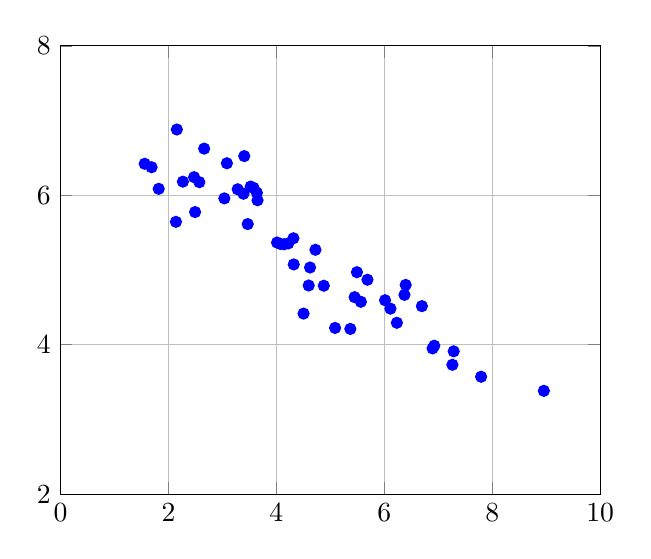
\begin{tikzpicture}
    \begin{axis}[
        xlabel={},
        ylabel={},
        xmin=0, xmax=10,
        ymin=2, ymax=8,
        grid=major,
        title={}
    ]

    % Define the data points for the scatter plot
    \addplot[only marks, mark=*, color=blue] table {
         x y
 6.895 3.95
 2.475 6.242
 3.283 6.08
 6.374 4.667
 5.566 4.574
 4.504 4.416
 2.494 5.775
 3.036 5.958
 1.82 6.086
 5.688 4.869
 8.957 3.382
 2.156 6.88
 3.469 5.614
 2.662 6.624
 4.22 5.355
 6.697 4.516
 7.794 3.571
 5.45 4.636
 4.316 5.424
 7.286 3.911
 3.639 6.033
 3.39 6.02
 4.624 5.033
 3.083 6.428
 4.724 5.27
 3.651 5.933
 3.577 6.099
 7.262 3.731
 4.077 5.348
 4.879 4.789
 5.088 4.224
 2.268 6.182
 6.114 4.482
 4.322 5.074
 5.493 4.97
 3.405 6.524
 1.56 6.421
 6.014 4.595
 4.599 4.792
 6.396 4.8
 1.688 6.375
 6.233 4.293
 6.926 3.986
 4.143 5.344
 2.573 6.175
 4.013 5.367
 2.139 5.644
 5.371 4.211
 3.524 6.116
    };

    %\addplot[color=red, thick, domain=1:9] expression {1.1*x + 1};

    \end{axis}
\end{tikzpicture}
\end{center}

The scatterplot gives a visual representation of the relationship between the two variables, and often if there's a strong association between the two variables, it's clearly visible. In this case, we can see that larger values of the variable on the horizontal axis are associated with smaller values of the variable on the vertical axis. The following definition gives a quantitative measure of this association.

\begin{definition}
The \newterm{correlation coefficient}\index{Correlation Coefficient} is defined, for populations and samples respectively, as

$$\rho = \frac{1}{n}\sum_{i=1}^{n}\left(\frac{x_i - \mu_x}{\sigma_x}\right)\left(\frac{y_i - \mu_y}{\sigma_y}\right) \qquad \text{and} \ \ \qquad r = \frac{1}{n-1}\sum_{i=1}^{n}\left(\frac{x_i - \overline{x}}{s_x}\right)\left(\frac{y_i - \overline{y}}{s_y}\right).$$

In both cases, it is the mean product of the $z$-scores, across all individuals in the dataset. Note that in the case of a sample, the sample standard deviation is used in place of the population standard deviation, and the result is not truly a mean, since we divide by $n-1$ instead of $n$, as when computing the sample variance.
\end{definition}

\begin{example}\label{CorrelationEx}
The math and reading grades in a random sample of five students from an elementary school are given below. Compute the coefficient of correlation, $r$.

\begin{center}
\begin{minipage}{0.4\textwidth}
\renewcommand{\arraystretch}{1.25}
\begin{center}
\begin{tabular}{|c|c|c|}
\hline
Name & Math Gr. & Read Gr. \\
\hline
Alice & $72$ & $84$ \\
\hline
Bob & $93$ & $82$  \\
\hline
Celia & $88$ & $91$  \\
\hline
Dave & $68$ & $75$  \\
\hline
Evan & $77$ & $73$  \\
\hline
\end{tabular}
\vspace*{0.1in}
\end{center}
\end{minipage}\begin{minipage}{0.4\textwidth}
\begin{center}
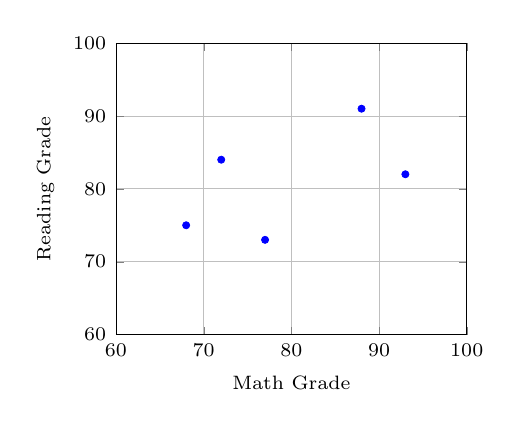
\begin{tikzpicture}[scale=0.65]
    \begin{axis}[
        xlabel={Math Grade},
        ylabel={Reading Grade},
        tick label style={font=\scriptsize, scale = 1/0.65},
        label style={font=\scriptsize, scale = 1/0.65},
        xmin=60, xmax=100,
        ymin=60, ymax=100,
        grid=major,
        title={}
    ]

    % Define the data points for the scatter plot
    \addplot[only marks, mark=*, color=blue] table {
        x y
        72 84
        93 82
        88 91
        68 75
        77 73
    };

    \end{axis}
\end{tikzpicture}
\end{center}
\end{minipage}
\end{center}

Note that we will compute the sample correlation, $r$, which implies we're actually interested in the association between the two variables in the population we're sampling from (all students at the school), not just the association observed in this particular group of five students.

The mean and standard deviation for math grades are $\overline{x} = 79.60$ and $s_x = 10.60$, and the mean and standard deviation for reading grades are $\overline{y} = 81.00$ and $s_y = 7.25$. Standardizing each of the values, then computing the product across each row, summing the results, and dividing by $n-1 = 4$,

\begin{center}
\begin{minipage}{0.32\textwidth}
\renewcommand{\arraystretch}{1.25}
\begin{center}
\begin{tabular}{|c|c|c|}
\hline
Name & Math Z & Read Z \\
\hline
Alice & $-0.72$ & $0.41$ \\
\hline
Bob & $1.26$ & $0.14$  \\
\hline
Celia & $0.79$ & $1.38$  \\
\hline
Dave & $-1.09$ & $-0.83$  \\
\hline
Evan & $-0.25$ & $-1.10$  \\
\hline
\end{tabular}
\vspace*{0.1in}
\end{center}
\end{minipage}\ \ \begin{minipage}{0.55\textwidth}
$\begin{aligned}r &= \textstyle\frac{1}{4}\sum_{i=1}^{5}z_{x_i}z_{y_i} \\
&= \textstyle\frac{1}{4}\left((-0.72)(0.41)+(1.26)(0.14)+ \dots + (-0.25)(-1.10)\right) \\
&= \textstyle\frac{1}{4} \cdot 2.68 \\ &= 0.54 \end{aligned}$
\end{minipage}
\end{center}
Thus, the sample correlation coefficient between math grades and reading grades is $r = 0.54$.
\end{example}

\begin{keypoint}
The coefficient of correlation is a measure of how well the points in the scatterplot line up along a straight line. There could be other clear patterns in the scatterplot, and the value of one variable can even be completely determined by the other, but we can still have $r = 0$, which is the case for each scatterplot below.
\end{keypoint}

\begin{center}
\begin{minipage}{0.33\textwidth}
\begin{center}
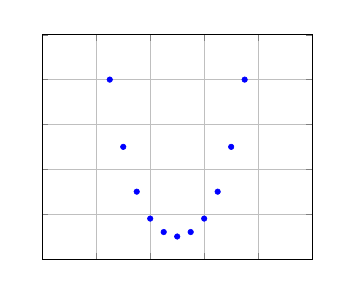
\begin{tikzpicture}[scale=0.5]
    \begin{axis}[
        tick label style={font=\scriptsize, scale = 1/0.65},
        label style={font=\scriptsize, scale = 1/0.65},
        xticklabel=\empty,
        yticklabel=\empty,
        xmin=0, xmax=100,
        ymin=0, ymax=100,
        grid=major,
        title={}
    ]

    % Define the data points for the scatter plot
    \addplot[only marks, mark=*, color=blue] table {
        x y
        50 10
        45 12
        55 12
        60 18
        40 18
        35 30
        65 30
        70 50
        30 50
        75 80
        25 80
            };

    \end{axis}
\end{tikzpicture}
\end{center}
\end{minipage}\begin{minipage}{0.33\textwidth}
\begin{center}
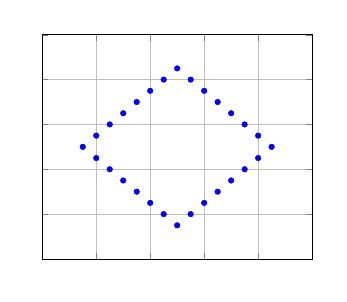
\begin{tikzpicture}[scale=0.5]
    \begin{axis}[
        tick label style={font=\scriptsize, scale = 1/0.65},
        label style={font=\scriptsize, scale = 1/0.65},
        xticklabel=\empty,
        yticklabel=\empty,
        xmin=0, xmax=100,
        ymin=0, ymax=100,
        grid=major,
        title={}
    ]

    % Define the data points for the scatter plot
    \addplot[only marks, mark=*, color=blue] table {
        x y
        15 50
        85 50
        20 55
        80 55
        20 45
        80 45
        25 60
        75 60
        25 40
        75 40
        30 35
        30 65
        70 35
        70 65
        35 70
        35 30
        65 70
        65 30
        40 75
        60 75
        40 25
        60 25
        45 80
        45 20
        55 80
        55 20
        50 85
        50 15
    };

    \end{axis}
\end{tikzpicture}
\end{center}
\end{minipage}\begin{minipage}{0.33\textwidth}
\begin{center}
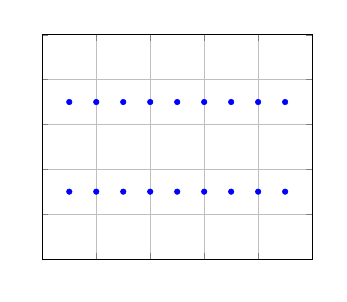
\begin{tikzpicture}[scale=0.5]
    \begin{axis}[
        tick label style={font=\scriptsize, scale = 1/0.65},
        label style={font=\scriptsize, scale = 1/0.65},
        xticklabel=\empty,
        yticklabel=\empty,
        xmin=0, xmax=100,
        ymin=0, ymax=100,
        grid=major,
        title={}
    ]

    % Define the data points for the scatter plot
    \addplot[only marks, mark=*, color=blue] table {
        x y
        10 70
        20 70
        30 70
        40 70
        50 70
        60 70
        70 70
        80 70
        90 70
        10 30
        20 30
        30 30
        40 30
        50 30
        60 30
        70 30
        80 30
        90 30
    };

    \end{axis}
\end{tikzpicture}
\end{center}
\end{minipage}
\end{center}

%\begin{proposition}
%The coefficient of correlation always takes a value in the interval $[-1,1]$, and takes the value $\pm 1$ if and only if all points in the scatterplot lie on a line of nonzero slope.
%\end{proposition}
%\begin{proof}

%\end{proof}

The coefficient of correlation measures the strength and direction of the linear relationship between the variables. The result is typically summarized with the terms strong, weak, positive, and negative. Two variables with $r = 0.32$ are weakly positively correlated, while two variables with $r=-0.83$ are strongly negatively correlated.

\begin{proposition}
The coefficient of correlation always takes a value in the interval $[-1,1]$, and takes the value $\pm 1$ if and only if all points in the scatterplot lie on a line (excepting the cases where the scatterplot contains only a single point, or the line is vertical or horizontal, in which case $r$ is undefined).
\end{proposition}

\begin{remark}
It's important to realize the presence of a strong correlation between variables does not imply any causal link between them, and even when there is such a link, what the nature of that link might be. A common cautionary tale involves a town where an analyst finds a strong positive correlation between the number of active fire trucks in an area, and the number of fires in that area. The town decides to take advantage of this result and prevent fires by decommissioning all of their fire trucks.
\end{remark}

Suppose we'd like to predict the value of one variable (which we'll the \newterm{response variable}\index{Response Variable}, $y$) using the value of the other (which we'll call the \newterm{explanatory variable}\index{Explanatory Variable}, $x$). In other words, we would like to find a function $f$ whose inputs are possible values of $x$ and whose outputs we can interpret as predicted values of $y$. This very general problem of constructing a function which models the relationship between a quantitative explanatory and response variable from a sample of points is known as \newterm{regression}. %In the next section, we'll study this problem in the special case where the function $f$ is restricted to being linear.

\section{The Least-Squares Regression Line}

Given a scatterplot, with the explanatory variable on the horizontal axis, and the response variable on the vertical axis, our goal is to find a function $f$ which best describes the relationship between the two variables. 

If we restrict the form of $f$ to a linear function $f(x) = ax+b$, and measure the degree to which $f$ deviates from the data by summing the squared differences between the values of the response variable $y_i$ and the value of $f(x_i)$ on the line (these differences are known as \newterm{residuals}\index{Residuals}, denoted $r_i$), we obtain the \newterm{least squares regression line}\index{Regression Line}.

\begin{center}
\begin{minipage}{0.35\textwidth}
\begin{center}
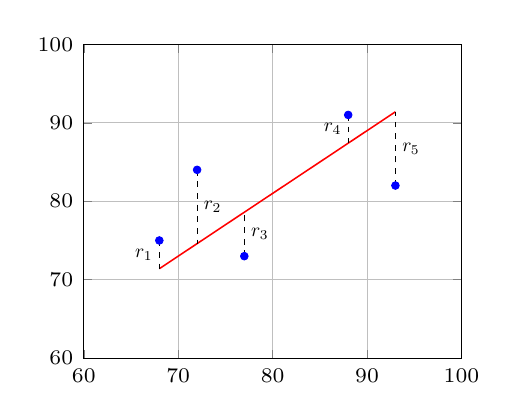
\begin{tikzpicture}[scale=0.7]
    \begin{axis}[
        xlabel={},
        ylabel={},
        tick label style={font=\scriptsize, scale = 1/0.65},
        label style={font=\scriptsize, scale = 1/0.65},
        xmin=60, xmax=100,
        ymin=60, ymax=100,
        grid=major,
        title={}
    ]

    % Define the data points for the scatter plot
    \addplot[only marks, mark=*, color=blue] table {
        x y
        72 84
        93 82
        88 91
        68 75
        77 73
    };
    
    \addplot[color=red, thick, domain=68:93] expression {0.8*x+17};
    \addplot [dashed] coordinates {(72,84) (72,0.8*72+17)} node[midway, right] {$r_2$};
    \addplot [dashed] coordinates {(93,82) (93,0.8*93+17)} node[midway, right] {$r_5$};
    \addplot [dashed] coordinates {(88,91) (88,0.8*88+17)} node[midway, left] {$r_4$};
    \addplot [dashed] coordinates {(68,75) (68,0.8*68+17)} node[midway, left] {$r_1$};
    \addplot [dashed] coordinates {(77,73) (77,0.8*77+17)} node[midway, right] {$r_3$};

    \end{axis}
\end{tikzpicture}

\end{center}
\end{minipage}\qquad\begin{minipage}{0.6\textwidth}
The least squares regression line $f(x) = ax + b$ is the line that results in the smallest possible sum of squared residuals
$$RSS = \sum_{i=1}^{n} r_i = \sum_{i=1}^{n} (y_i - f(x_i))^2$$
across all $a, b \in \mathbb{R}$. Using techniques from linear algebra or multivariable calculus, it's possible to solve for the values of $a$ and $b$ in general. Doing so yields the result below.
\end{minipage}
\end{center}

\begin{proposition}\label{RegressionLineEq}
Given a sample of points $(x_1, y_1)$, $(x_2, y_2)$, \dots , $(x_n, y_n)$, the least squares regression line $f(x) = ax+b$ has slope $a = r \cdot \frac{s_y}{s_x}$ and y-intercept $b = \overline{y} - a\cdot\overline{x}$.
\end{proposition}

\begin{remark}
To write the equation of the regression line requires calculating $\overline{x}$, $\overline{y}$, $s_x$, $s_y$, and $r$. This means that if we've gone through the trouble of computing the coefficient of correlation, the equation of the regression line comes essentially for free.
\end{remark}

\begin{example}\label{GradesRegressionEx} Find the equation of the least squares regression line for the data below (this is the data from Example \ref{CorrelationEx}), using math grade as the explanatory variable, and reading grade as the response variable. Use the line to find the predicted reading grade for a student whose math grade is 91.

\begin{center}
\begin{minipage}{0.4\textwidth}
\renewcommand{\arraystretch}{1.25}
\begin{center}
\begin{tabular}{|c|c|c|}
\hline
Name & Math Gr. & Read Gr. \\
\hline
Alice & $72$ & $84$ \\
\hline
Bob & $93$ & $82$  \\
\hline
Celia & $88$ & $91$  \\
\hline
Dave & $68$ & $75$  \\
\hline
Evan & $77$ & $73$  \\
\hline
\end{tabular}
\vspace*{0.1in}
\end{center}
\end{minipage}\begin{minipage}{0.4\textwidth}
\begin{center}
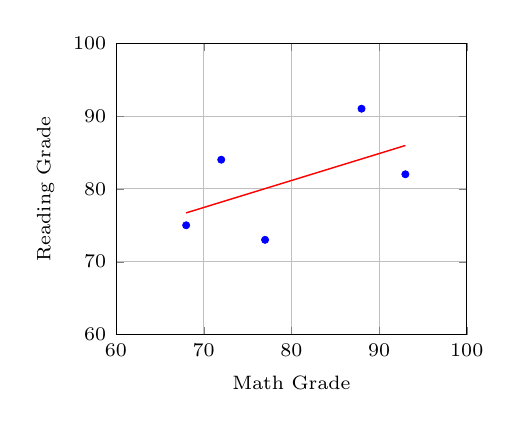
\begin{tikzpicture}[scale=0.65]
    \begin{axis}[
        xlabel={Math Grade},
        ylabel={Reading Grade},
        tick label style={font=\scriptsize, scale = 1/0.65},
        label style={font=\scriptsize, scale = 1/0.65},
        xmin=60, xmax=100,
        ymin=60, ymax=100,
        grid=major,
        title={}
    ]

    % Define the data points for the scatter plot
    \addplot[only marks, mark=*, color=blue] table {
        x y
        72 84
        93 82
        88 91
        68 75
        77 73
    };
    
    \addplot[color=red, thick, domain=68:93] expression {0.37*x+51.54};

    \end{axis}
\end{tikzpicture}
\end{center}
\end{minipage}
\end{center}

In Example \ref{CorrelationEx}, we computed $\overline{x} = 79.60$, $\overline{y} = 81.00$, $s_x = 10.60$, $s_y = 7.25$, and $r = 0.64$, so we can calculate $a = 0.54 \cdot \frac{7.25}{10.60} = 0.37$ and $b = 81.00 - 0.37 \cdot 79.60 = 51.54$. Thus, the equation of the regression line is $f(x) = 0.37x+51.54$, which is shown on the scatterplot above.

Using the regression line, we can compute a predicted reading grade of $\widehat{y} = 0.38\cdot 91 + 51.54 \approx 86$ for a student whose math grade is 91. 
\end{example}

We use the notation $\widehat{y}$ to indicate a predicted value of the response variable from the regression line. In particular, if $(x_i, y_i)$ is one of the points in our sample data, then it's important to distinguish the observed value $y_i$ in the sample data from the predicted value $\widehat{y}_i = f(x_i)$, and with this notation we can write the residual $r_i$ as the difference $y_i - \widehat{y}_i$.

\begin{remark}
The domain of the regression line is restricted to values of the explanatory variable inside the range of the sample data. Using the regression line to make predictions outside the range of the sample data is known as \newterm{extrapolation}\index{Extrapolation}, and should always be avoided.
\end{remark}

Note that the slope of the regression line can be interpreted as the expected change in the response variable when the explanatory variable's value increases by one, though one has to be careful to avoid assuming any causal link between the values of the two. 

In some cases, like Example \ref{PlantsRegressionEx} below, we would expect that we can exert some degree of control over the value of the response variable by altering the explanatory variable. In others instances, like Example \ref{GradesRegressionEx} above, this may not be the case (despite the positive correlation between the grades, spending extra study time on math in order to obtain a higher grade could cause a student's reading grade to suffer).

\begin{example}\label{PlantsRegressionEx}
Twelve plants are grown under identical conditions, but with the amount of fertilizer used in the soil each grows in carefully controlled. The amount of fertilizer mixed into the soil when the plants are potted and the height of the plants after four weeks of growth are recorded in the table below.

\renewcommand{\arraystretch}{1.25}
\begin{center}
\begin{tabular}{|c|c|c|c|c|c|c|c|c|c|c|c|c|}
\hline
Fertilizer\,(g) & $15$ & $25$ & $20$ & $25$ & $40$ & $35$ & $30$ & $40$ & $45$ & $20$ & $30$  \\
\hline
Height\,(cm) & $14$ & $17$ & $18$ & $22$ & $27$ & $24$ & $24$ & $28$ & $28$ & $23$ & $26$   \\
\hline
\end{tabular}
\end{center}

Find the equation of the least squares regression line, using the amount of fertilizer as the explanatory variable and the height as the response variable, and interpret its slope in this context. What does the regression line predict the height of a plant grown in soil with 32\,g of fertilizer will be?

After computing $\overline{x} = 29.55$, $s_x = 9.61$, $\overline{y} = 22.82$, $s_y = 4.69$, and $r = 0.86$, we can then calculate $a = 0.86\cdot\frac{4.69}{9.61} = 0.42$ and $b = 22.82-0.42\cdot29.55 = 10.41$, and arrive at the equation $\widehat{y} = 0.42x+10.41$.

The slope of the line, 0.42, corresponds to the additional height predicted to result from using one extra gram of fertilizer. Of course, in practice one extra gram of fertilizer has a larger effect in under-fertilized soil than in well-fertilized soil, and at some point adding more fertilizer will do more harm than good. Nonetheless, the slope provides a summary of the effect of fertilizer in our linear model, within the range of the sample data.

If we let $x = 32$, the model predicts the height will be $\widehat{y} = 0.42\cdot 32 + 10.41 = 23.85\, cm$.
\end{example}

%There is a more efficient formula for the slope of the regression line which is useful in the case where the coefficient of correlation is not already known, and will be useful in the next section.

%\begin{proposition}\label{RegressionSlopeFormula}
%The slope of the regression line is given by $a = \displaystyle\frac{\sum_{i=1}^{n}(x_i-\overline{x})(y_i-\overline{y})}{\sum_{i=1}^{n}(x_i-\overline{x})^2}$.
%\end{proposition}

%\begin{proof}
%In Proposition \ref{RegressionLineEq} earlier, we have the expression $a = r\cdot\frac{s_y}{s_x}$ for the slope, and
%$$\begin{aligned}r\cdot\frac{s_y}{s_x} &= \frac{1}{n-1}\left(\sum_{i=1}^{n}\frac{(x_i-\overline{x})}{s_x}\frac{(y_i-\overline{y})}{s_y}\right)\cdot \frac{s_y}{s_x} \\ 
%&= \frac{s_y}{s_x}\cdot\frac{1}{n-1}\cdot\frac{1}{s_x s_y}\sum_{i=1}^{n}(x_i-\overline{x})(y_i-\overline{y}) \\ 
%&= \frac{1}{(n-1)s^2_x}\cdot\sum_{i=1}^{n}(x_i-\overline{x})(y_i-\overline{y}) \\ 
%&= \frac{1}{(n-1)\frac{1}{n-1}\sum_{i=1}^{n}(x_i-\overline{x})^2}\cdot\sum_{i=1}^{n}(x_i-\overline{x})(y_i-\overline{y}) \\[1ex]
%&= \frac{\sum_{i=1}^{n}(x_i-\overline{x})(y_i-\overline{y})}{\sum_{i=1}^{n}(x_i-\overline{x})^2} \\ \end{aligned}$$
%\end{proof}

\section{The Coefficient of Determination}

Now that we can find the equation of the regression line and use it to make predictions, our next concern is how to measure how useful the line actually is. One natural way to quantify this is to ask how much better the line is than a simpler alternative, always predicting the mean value of $y$. This should sound familiar, since what we're really doing here is comparing the regression line to a simpler model where the explanatory variable has \emph{no effect} on the value of the response variable.

\begin{definition}
The \newterm{total sum of squares}\index{TSS} is the sum of the squared differences between the observed values of the response variable and the mean value, and the \newterm{explained sum of squares}\index{ESS} is the sum of the squared differences between the predicted values of the response variable and the mean value.
$$TSS = \sum_{i=1}^{n} (y_i - \overline{y})^2 \qquad ESS = \sum_{i=1}^{n} (\widehat{y_i} - \overline{y})^2$$
\end{definition}
\begin{center}
\begin{minipage}{0.45\textwidth}
\begin{center}
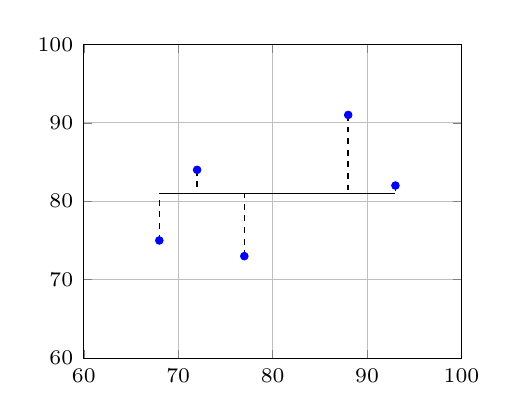
\begin{tikzpicture}[scale=0.7]
    \begin{axis}[
        xlabel={},
        ylabel={},
        tick label style={font=\scriptsize, scale = 1/0.65},
        label style={font=\scriptsize, scale = 1/0.65},
        xmin=60, xmax=100,
        ymin=60, ymax=100,
        grid=major,
        title={}
    ]

    % Define the data points for the scatter plot
    \addplot[only marks, mark=*, color=blue] table {
        x y
        72 84
        93 82
        88 91
        68 75
        77 73
    };
    
    \addplot[color=black, thick, domain=68:93] expression {81};
    \addplot [dashed,thick] coordinates {(72,84) (72,81)} node[midway, right] {};
    \addplot [dashed,thick] coordinates {(93,82) (93,81)} node[midway, right] {};
    \addplot [dashed,thick] coordinates {(88,91) (88,81)} node[midway, left] {};
    \addplot [dashed,thick] coordinates {(68,75) (68,81)} node[midway, left] {};
    \addplot [dashed,thick] coordinates {(77,73) (77,81)} node[midway, right] {};

    \end{axis}
\end{tikzpicture}

\end{center}
\end{minipage}\qquad\begin{minipage}{0.45\textwidth}
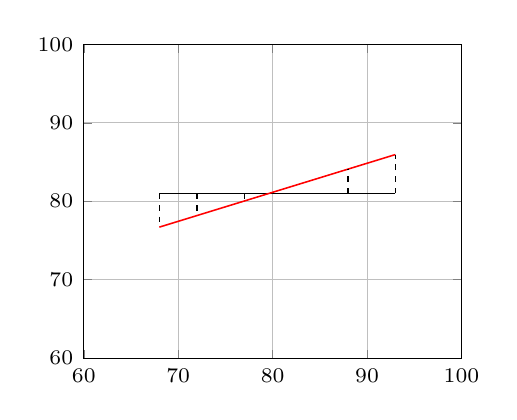
\begin{tikzpicture}[scale=0.7]
    \begin{axis}[
        xlabel={},
        ylabel={},
        tick label style={font=\scriptsize, scale = 1/0.65},
        label style={font=\scriptsize, scale = 1/0.65},
        xmin=60, xmax=100,
        ymin=60, ymax=100,
        grid=major,
        title={}
    ]

    % Define the data points for the scatter plot
    %\addplot[only marks, mark=*, color=blue] table {
    %    x y
    %    72 84
    %    93 82
    %    88 91
    %    68 75
    %    77 73
    %};
    
    \addplot[color=black, thick, domain=68:93] expression {81};
    \addplot[color=red, thick, domain=68:93] expression {0.37*x+51.54};
    \addplot [dashed,thick] coordinates {(72,81) (72,0.37*72+51.54)} node[midway, right] {};
    \addplot [dashed,thick] coordinates {(93,81) (93,0.37*93+51.54)} node[midway, right] {};
    \addplot [dashed,thick] coordinates {(88,81) (88,0.37*88+51.54)} node[midway, left] {};
    \addplot [dashed,thick] coordinates {(68,81) (68,0.37*68+51.54)} node[midway, left] {};
    \addplot [dashed,thick] coordinates {(77,81) (77,0.37*77+51.54)} node[midway, right] {};

    \end{axis}
\end{tikzpicture}
\end{minipage}
\end{center}

\begin{keypoint}
The $TSS$ measures of the total amount of variation of the response variable around its mean. Notice the similarity between the $TSS$ and the sample variance (they differ only by factor of $n-1$). The $ESS$ measures the amount of variation from the mean which is accounted for by the regression line.
\end{keypoint}

If the sample points fall almost exactly along a straight line, then the $TSS$ and $ESS$ will be almost the same. In general, the higher the proportion of variation from the mean the regression line accounts for, the better it fits the data.  This motivates the definition below.

\begin{center}
\begin{minipage}{0.45\textwidth}
\begin{center}
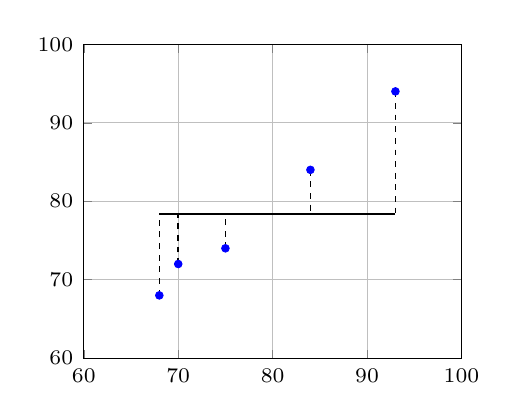
\begin{tikzpicture}[scale=0.7]
    \begin{axis}[
        xlabel={},
        ylabel={},
        tick label style={font=\scriptsize, scale = 1/0.65},
        label style={font=\scriptsize, scale = 1/0.65},
        xmin=60, xmax=100,
        ymin=60, ymax=100,
        grid=major,
        title={}
    ]

    % Define the data points for the scatter plot
    \addplot[only marks, mark=*, color=blue] table {
        x y
        68 68
        70 72
        75 74
        84 84
        93 94
    };
    
    \addplot[color=black, thick, domain=68:93] expression {78.4};
    \addplot [dashed,thick] coordinates {(68,68) (68,78.4)} node[midway, right] {};
    \addplot [dashed,thick] coordinates {(70,72) (70,78.4)} node[midway, right] {};
    \addplot [dashed,thick] coordinates {(75,74) (75,78.4)} node[midway, left] {};
    \addplot [dashed,thick] coordinates {(84,84) (84,78.4)} node[midway, left] {};
    \addplot [dashed,thick] coordinates {(93,94) (93,78.4)} node[midway, right] {};

    \end{axis}
\end{tikzpicture}

\end{center}
\end{minipage}\qquad\begin{minipage}{0.45\textwidth}
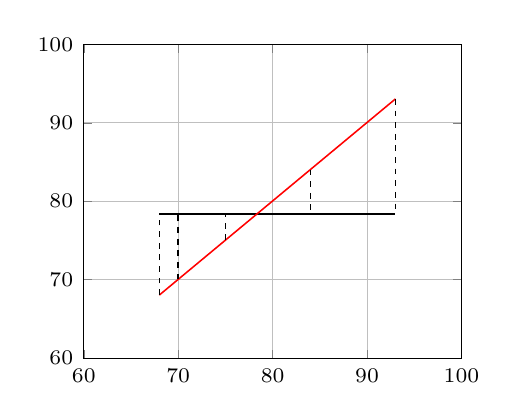
\begin{tikzpicture}[scale=0.7]
    \begin{axis}[
        xlabel={},
        ylabel={},
        tick label style={font=\scriptsize, scale = 1/0.65},
        label style={font=\scriptsize, scale = 1/0.65},
        xmin=60, xmax=100,
        ymin=60, ymax=100,
        grid=major,
        title={}
    ]

    % Define the data points for the scatter plot
    % Define the data points for the scatter plot
    %\addplot[only marks, mark=*, color=blue] table {
    %    x y
    %    68 68
    %    70 72
    %    75 74
    %    84 84
    %    93 94
    %};
    
    \addplot[color=black, thick, domain=68:93] expression {78.4};
    \addplot[color=red, thick, domain=68:93] expression {x+0.04055};
    \addplot [dashed,thick] coordinates {(68,68+0.04055) (68,78.4)} node[midway, right] {};
    \addplot [dashed,thick] coordinates {(70,70+0.04055) (70,78.4)} node[midway, right] {};
    \addplot [dashed,thick] coordinates {(75,75+0.04055) (75,78.4)} node[midway, left] {};
    \addplot [dashed,thick] coordinates {(84,84+0.04055) (84,78.4)} node[midway, left] {};
    \addplot [dashed,thick] coordinates {(93,93+0.04055) (93,78.4)} node[midway, right] {};

    \end{axis}
\end{tikzpicture}
\end{minipage}
\end{center}

\begin{definition} 
The \newterm{coefficient of determination}\index{Coefficient of Determination} is given by $R^2 = \frac{ESS}{TSS}$. It measures the proportion of the variance of the response variable which is captured by the regression line.
\end{definition}

\begin{theorem}
The coefficient of determination is the square of the coefficient of correlation, $R^2 = r^2$.
\end{theorem}
\begin{proof}
$$\begin{aligned} R^2 &= \frac{ESS}{TSS}
= \frac{\sum_{i=1}^{n}(\widehat{y}_i - \overline{y})^2}{\sum_{i=1}^{n}(y_i - \overline{y})^2} 
= \frac{\sum_{i=1}^{n}(ax_i+b - \overline{y})^2}{\sum_{i=1}^{n}(y_i - \overline{y})^2}
= \frac{\sum_{i=1}^{n}(r\frac{s_y}{s_x} x_i + \overline{y} - r\frac{s_y}{s_x}\overline{x} - \overline{y})^2}{\sum_{i=1}^{n}(y_i - \overline{y})^2} \\[2ex] 
&= \frac{\sum_{i=1}^{n}(r\frac{s_y}{s_x}(x_i - \overline{x}))^2}{\sum_{i=1}^{n}(y_i - \overline{y})^2} = r^2\frac{{s_y}^2}{{s_x}^2} \frac{\sum_{i=1}^{n}(x_i - \overline{x})^2}{\sum_{i=1}^{n}(y_i - \overline{y})^2} = r^2\frac{{s_y}^2}{{s_x}^2} \frac{(n-1){s_x}^2}{(n-1){s_y}^2} = r^2 \end{aligned}$$
\end{proof}

This means that if we have done the work of calculating the coefficient of correlation $r$, not only can we easily write down the equation of the regression line, we also get a quantitative measure of how well it fits the data.

\begin{example}
Calculate the coefficient of determination in Examples \ref{GradesRegressionEx} and \ref{PlantsRegressionEx}. In which case is the regression line a more informative model?

In Example \ref{GradesRegressionEx}, the regression line was $\widehat{y} = 0.37x+51.54$ with $r = 0.54$. Here, $r^2 = 0.29$, so only 29\% of the variance in reading grades is explained by the regression line.

In Example \ref{PlantsRegressionEx}, the regression line was $\widehat{y} = 0.42x+10.41$ with $r = 0.86$. Here, $r^2 = 0.74$, so here 74\% of the variance in height is explained by the regression line, and the regression line is a much better predictive model.
\end{example}

\begin{example}
In a study of user preferences, the number of comedy movies and horror movies watched by a sample of twelve users of a streaming service in the past year was recorded. The results are given in the table below.

\renewcommand{\arraystretch}{1.25}
\begin{center}
\begin{tabular}{|c|c|c|c|c|c|c|c|c|c|c|c|c|}
\hline
Comedy & $4$ & $12$ & $15$ & $1$ & $8$ & $5$ & $10$ & $9$ & $14$ & $1$ & $8$ & $8$  \\
\hline
Horror & $6$ & $9$ & $8$ & $9$ & $2$ & $7$ & $4$ & $8$ & $3$ & $13$ & $9$ & $2$   \\
\hline
\end{tabular}
\end{center}

Does it seem like the least squares regression line would be a useful model for predicting the number of horror movies users view from the number of comedy movies?

If we compute $r = -0.39$ and $r^2 = 0.15$, we can see there is a weak negative correlation between the two variables, but only 15\% of the variance in the number of comedies would be captured by the regression line, so it seems that the regression line would not be a very useful predictive model in this scenario.
\end{example}

%\begin{theorem} $SST = SSE + SSR$ \end{theorem}

%\begin{proof}
%By adding and subtracting the predicted values $\widehat{y}_i$ in the expression for the $SST$ and expanding, we can decompose the $SST$ into three terms as follows.
%$$\begin{aligned}SST &= \sum_{i=1}^{n}(y_i - \overline{y})^2 \\
%&= \sum_{i=1}^{n}(y_i - \widehat{y}_i + \widehat{y}_i - \overline{y})^2 \\
%&= \sum_{i=1}^{n}(y_i - \widehat{y}_i)^2 + 2(y_i - \widehat{y}_i)(\widehat{y}_i - \overline{y}) + (\widehat{y}_i - \overline{y})^2 \\
%&= \sum_{i=1}^{n}(y_i - \widehat{y}_i)^2 + \sum_{i=1}^{n} (\widehat{y}_i - \overline{y})^2 + 2\sum_{i=1}^{n}(y_i - \widehat{y}_i)(\widehat{y}_i - \overline{y}) \\ 
%& = SSR + SSE + 2\sum_{i=1}^{n}(y_i - \widehat{y}_i)(\widehat{y}_i - \overline{y}) \end{aligned}$$
%It now suffices to show that the last term is zero. To do this, recall that the equation of the least squares regression line is $\widehat{y} = ax + (\overline{y} - a\overline{x})$, which we can rearrange to $\widehat{y} - \overline{y} = a(x - \overline{x})$. Thus, for any $(x_i,y_i)$ in our sample, we have $\widehat{y}_i - \overline{y} = a(x_i - \overline{x})$ and
%$$(y_i - \widehat{y}_i) = (y_i - \widehat{y}_i) - \overline{y} + \overline{y} = (y_i-\overline{y}) - (\widehat{y}_i - \overline{y}) = (y_i - \overline{y})-a(x_i - \overline{x})$$
%We can use these relationships to eliminate all the predicted values of $y$ in the last term in our sum,
%$$\begin{aligned}\sum_{i=1}^{n}(y_i - \widehat{y}_i)(\widehat{y}_i - \overline{y}) &= \sum_{i=1}^{n}((y_i - \overline{y}) - a(x_i - \overline{x}))a(x_i - \overline{x}) \\
%&= a \sum_{i=1}^{n} (x_i - \overline{x})(y_i - \overline{y}) -a(x_i-\overline{x})^2 \\
%&= a \left(\sum_{i=1}^{n} (x_i - \overline{x})(y_i - \overline{y}) - a\sum_{i=1}^{n}(x_i-\overline{x})^2\right) \\
%&= a \left(\sum_{i=1}^{n} (x_i - \overline{x})(y_i - \overline{y}) - \frac{\sum_{i=1}^{n}(x_i-\overline{x})(y_i-\overline{y})}{\sum_{i=1}^{n}(x_i-\overline{x})^2}\sum_{i=1}^{n}(x_i-\overline{x})^2\right) \\ 
%&= a \left(\sum_{i=1}^{n} (x_i - \overline{x})(y_i - \overline{y}) - \sum_{i=1}^{n}(x_i-\overline{x})(y_i-\overline{y})\right) = 0\\ \end{aligned} $$
%Note the use of Proposition \ref{RegressionSlopeFormula} in the second last line.

%\end{proof}




